% !TeX root = ../tesis.tex

\section{Eritrocito sano}
\label{section:Res_Eritrocito_Sano}
Se consideró como modelo de un eritrocito sano a un óvalo de Cassini con valores de , como el mostrado en la Fig. Se consideró como material la función dieléctrica correspondiente a una concentración de 30.6 g/dL e inmersa en plasma con una epsilon de 1.823. En la Fig. se muestra la distribución del patrón de esparcimiento en el égimen de campo lejano, donde se emplea el valor del esparcimiento en escala logarítmica con unidades de decibelios. que indica el color y la forma del patrón indica la distribución. Se observa que el esparcimiento frontal posee la mayor intensidad, seguido del lateral y finalmente el retroesparcimiento. En la Fig. se muestra la gráfica polar del patrón de esparcimiento en donde se empleó la simetría alrededor del eje x para graficarlo y en la Fig. se muestra la gráfica cartesiana 
%
\begin{figure}[h!]
	\centering
		\sidesubfloat[Second image]{\hspace{-0.3cm}{
			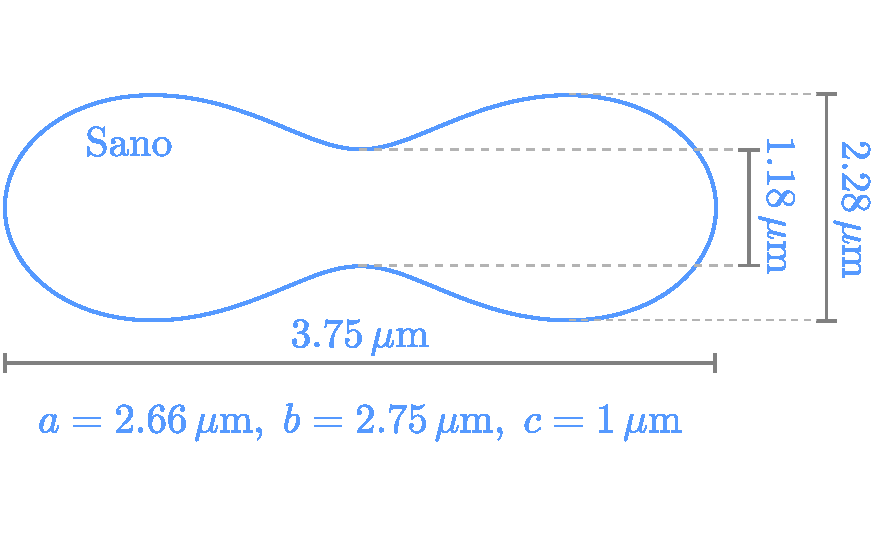
\includegraphics[width=0.45\textwidth]{../../Figuras/4-Resultados/Eritrocito_sano_corte.pdf}\label{subfig:FIT_cell_electric}}}\hspace{0.1cm}
	\sidesubfloat[First image]{\hspace{-0.5cm}{	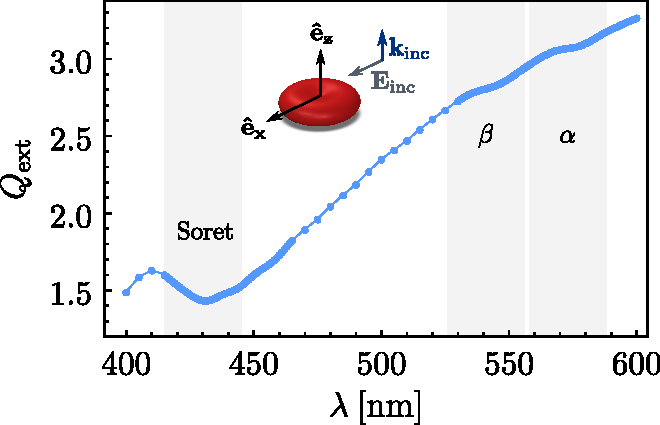
\includegraphics[width=0.45\textwidth]{../../Figuras/4-Resultados/Qext_EriSano.pdf}\label{subfig:FIT_cell_magnetic}}}
\vspace{-0.1cm}
	\caption{}
	\label{fig:FIT_cell}
\end{figure}
%



%
\begin{figure}[h!]
	\centering
	\sidesubfloat[First image]{\hspace{-0.5cm}{	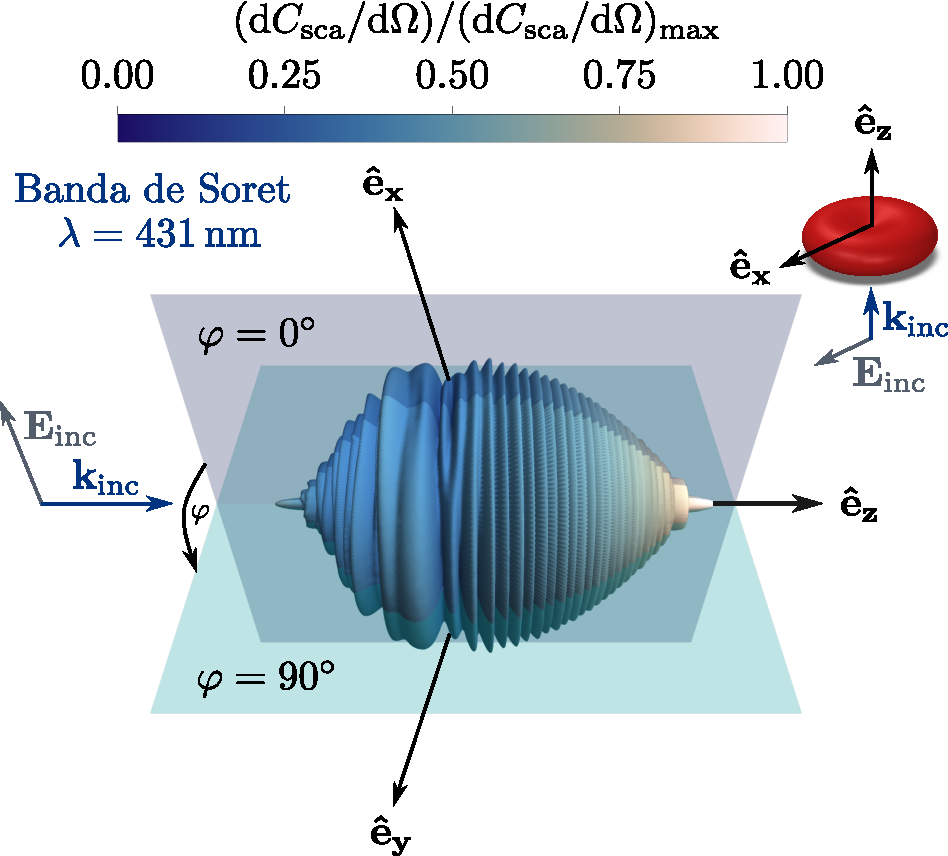
\includegraphics[width=7.3cm]{../../Figuras/4-Resultados/FFdistribution431_EriSano.pdf}\label{subfig:FIT_cell_magnetic}}}\hspace{0.1cm}
	\sidesubfloat[Second image]{\hspace{-0.5cm}{
			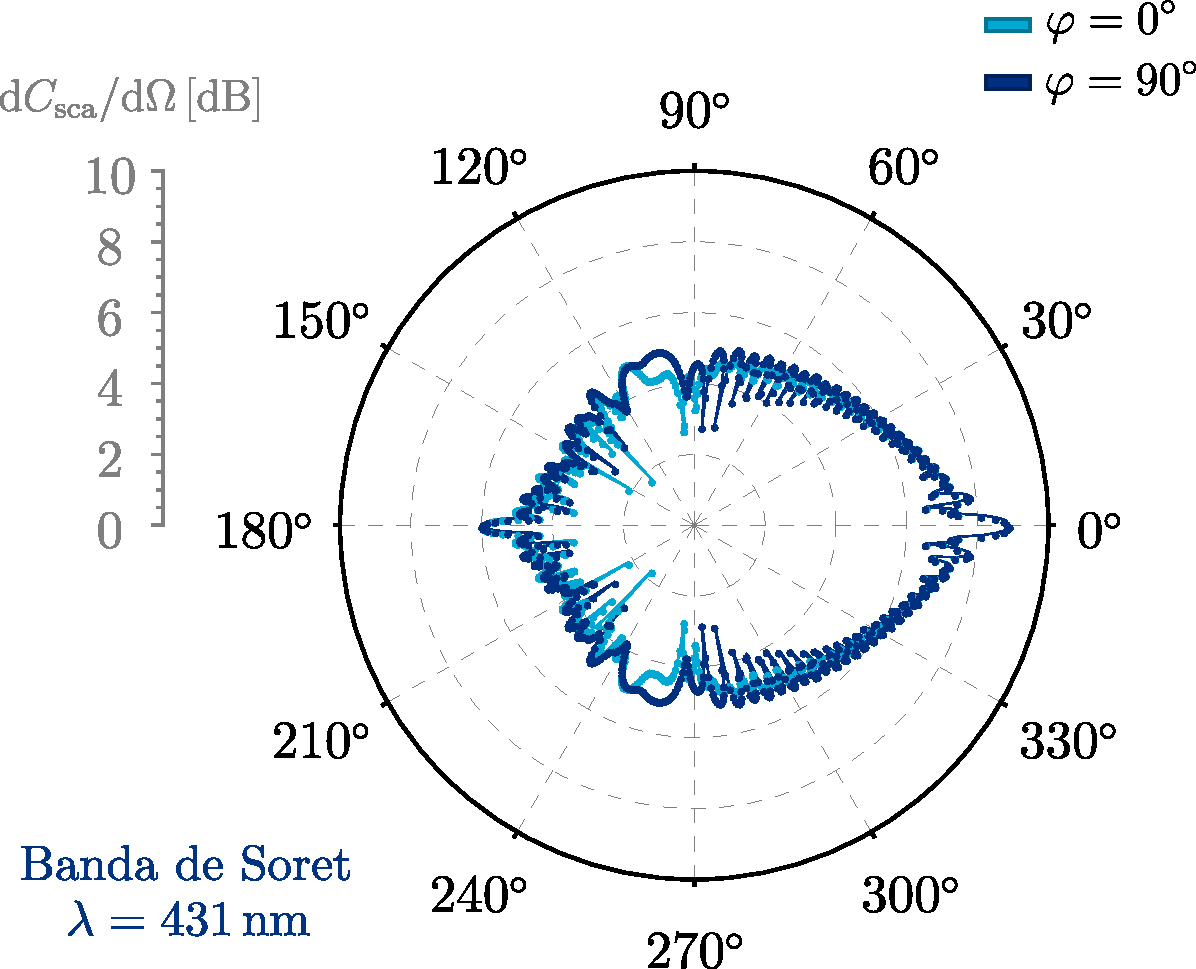
\includegraphics[width=8cm]{../../Figuras/4-Resultados/polarplot431FF_EriSano.pdf}\label{subfig:FIT_cell_electric}}}\vspace{-0.1cm}
	\\
	\vspace{0.1cm}
	
	\sidesubfloat[Third image]{\hspace{0.3cm}{
			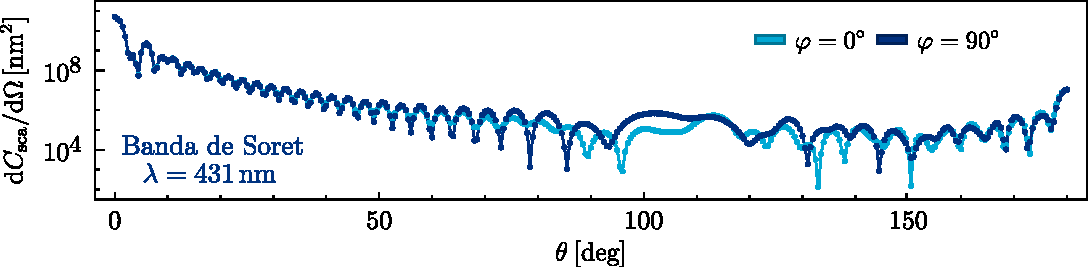
\includegraphics[width=14.8cm]{../../Figuras/4-Resultados/linearplot431FF_EriSano.pdf}\label{subfig:FIT_cell_electric}}}\vspace{-0.1cm}
	\caption{\textbf{a)} }
	\label{fig:FIT_cell}
\end{figure}
%




